%\section{Perceptron}
\label{sec:application:feedforward}

This section outlines how we have applied static feedfoward networks to our time series. For this purpose we used the MatLab toolbox for neural networks.

\subsection{Perceptron}
\label{subsec:perceptronapplication}

As a first attempt, we evaluated the Perceptron shown in \figref{perceptronnn}. 
It consists on a neuron with:
a number of set inputs equals to the amount of physiologycal signals, 
the hyperbolic tangent sigmoid as activation function
and $\text{bias}=0$. As Perceptrons are static (\ie, without memory), each time series is truncated in every step with a window length of 15 samples. 
With the set of samples formed by the all the input signals, an unique output sample is computed.
\begin{figure}[!ht]
\centering
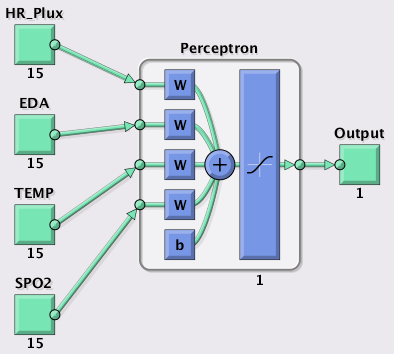
\includegraphics[width=0.5\columnwidth]{images/results/perceptronnn}
\caption{Perceptron neuron evaluated}
\label{fig:perceptronnn}
\end{figure}

As we could imagine, the results differ hugely from the desired behaviour of the network: we can see in the example depicted in \figref{perceptronResults}) how the Perceptron output is not capable of ``following'' the target signal.
Also reducing the set of physiological signals used as inputs or changing the length of their time-window, we obtained the similar ones.
\begin{figure}[!ht]
\centering
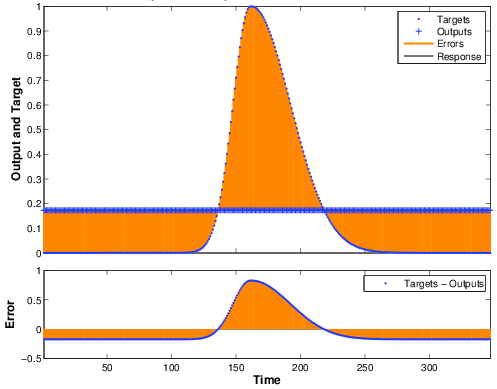
\includegraphics[width=0.7\columnwidth]{images/results/perceptronResults}
\caption{Example of the Perceptron neuron results}
\label{fig:perceptronResults}
\end{figure}


\subsection{Multilayer Perceptron}
\label{subsec:mlpapplication}
????????????


